\documentclass{article}
\usepackage{amsmath}
\usepackage{graphicx}
\usepackage{caption}
\usepackage{tikz}
\usepackage{hyperref}
\usepackage{listings}
\usepackage{color}

\title{Optimization of Supply Chain Routing for Material Supply Management}
\author{Ahmad Iftikhar Khan, Anoop Nair, Dipendra Gautam }
\date{}

\begin{document}

\maketitle

\section{Introduction}

Efficient route optimization is required to reduce transportation costs and ensure timely delivery of goods. The objective of this study is to deploy a linear optimization model to minimize the total transportation costs of goods from supply nodes (warehouses) to demand nodes. The approach uses mixed integer linear programming (MIP) to solve the material supply problem, integrating multiple factors such as freight rates, transportation capacity, and warehouse costs. The approach takes into account both the supply constraints from various warehouses and the demand from different projects to find the optimal transportation routes.

\section{Data Preprocessing}


\begin{figure}[!h]
     \begin{center}
     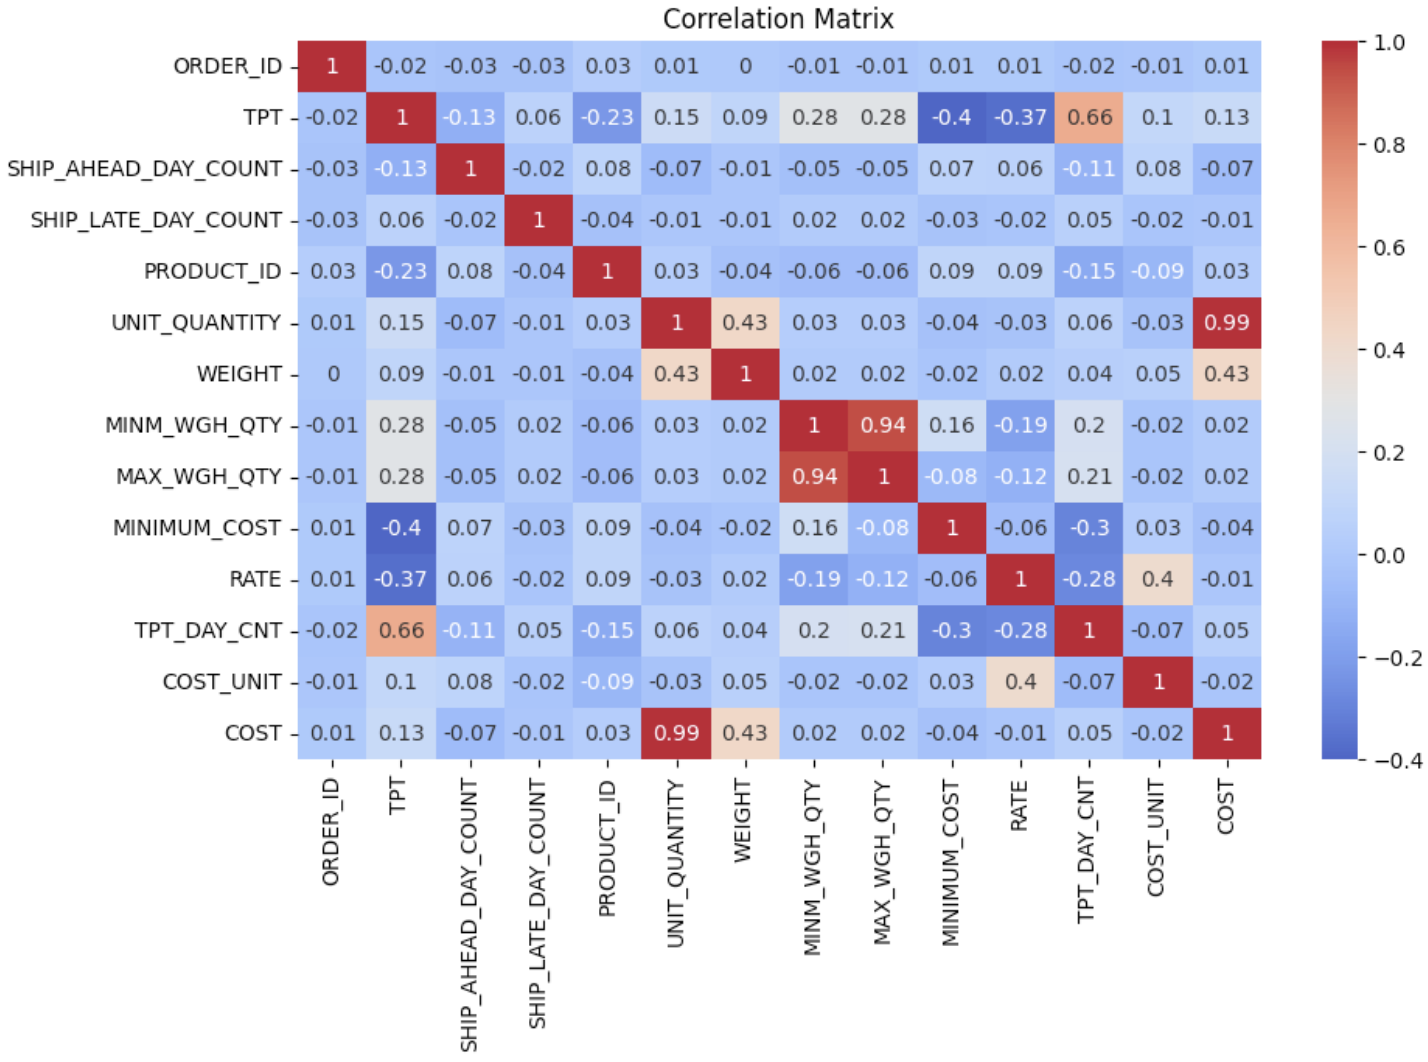
\includegraphics[width=0.6\paperwidth]{correlation.png}
     \end{center}
     \caption{Correlation matrix}
     \label{fig:cd}
\end{figure}




\begin{figure}[!h]
     \begin{center}
     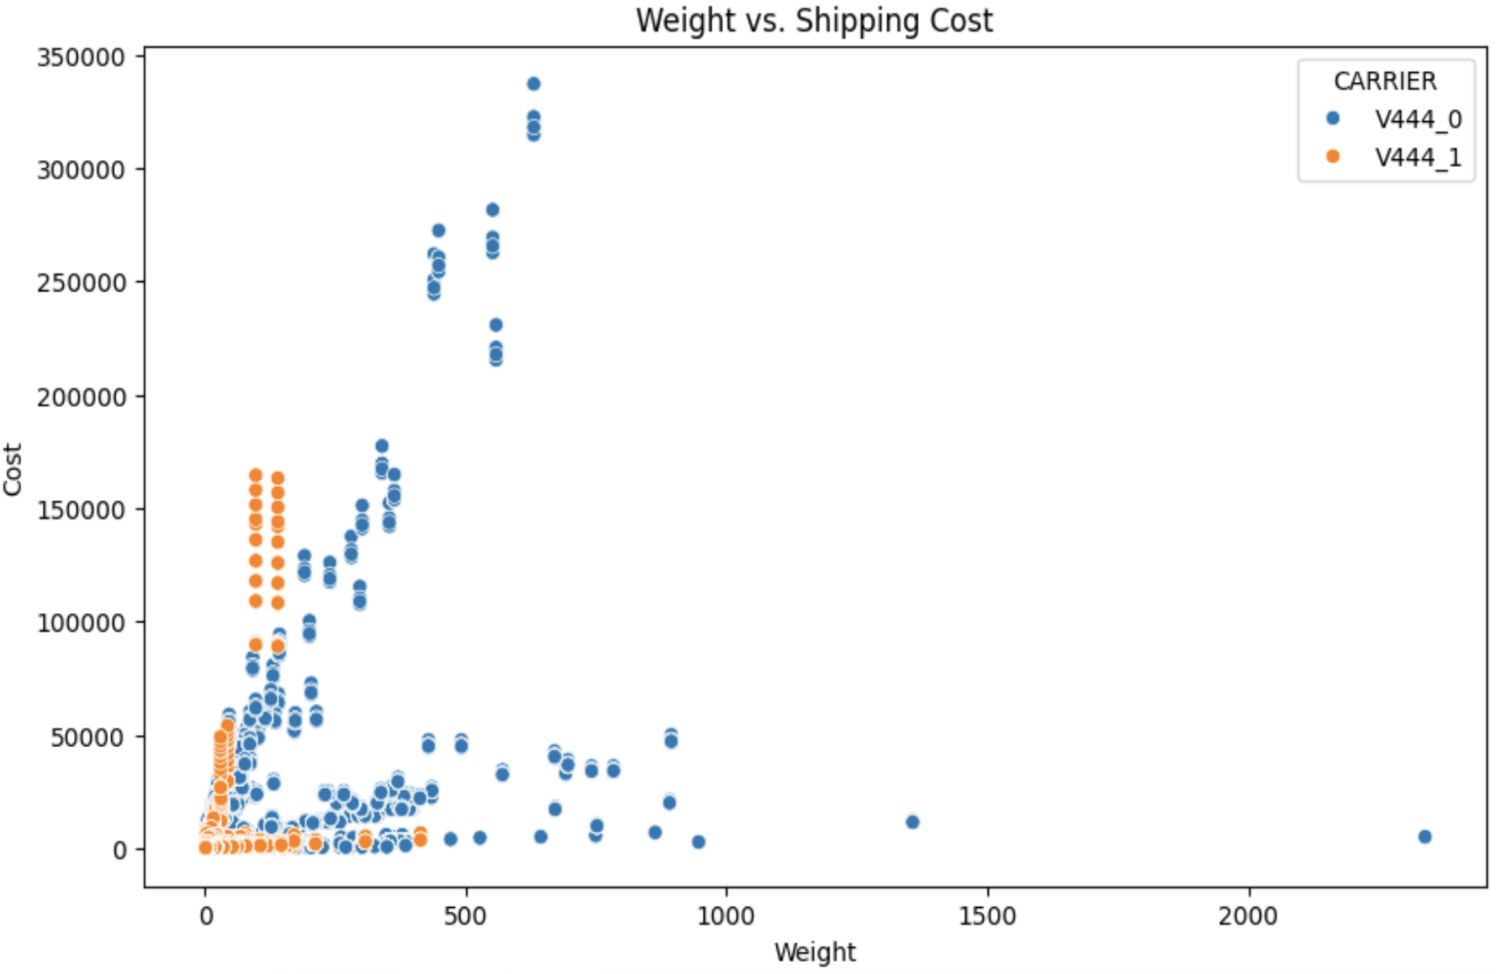
\includegraphics[width=0.6\paperwidth]{scatterplot.png}
     \end{center}
     \caption{Cost analysis of two carriers}
     \label{fig:cd}
\end{figure}


The data for this study was sourced from an Excel file titled \texttt{"Supply chain logistics problem.xlsx"}, which contained several sheets including \texttt{OrderList}, \texttt{FreightRates}, \texttt{WhCosts}, and \texttt{WhCapacities}. Initially, data cleaning is done and preprocessing is conducted to handle any inconsistencies, missing values, and duplicate entries. The following steps are considered:

\begin{itemize}
    \item \textbf{Redundant data:} Duplicate entries were removed to ensure data integrity, particularly in the \texttt{FreightRates} data frame.
    \item \textbf{Missing Value:} Rows with missing values were dropped from the datasets, ensuring that only complete data was used in the analysis.
    \item \textbf{Column Renaming:} Columns in each data frame were standardized by stripping leading and trailing spaces, replacing spaces with underscores, and converting all column names to uppercase for uniformity.
\end{itemize}

\section{Exploratory Data Analysis}



\begin{figure}[!h]
     \begin{center}
     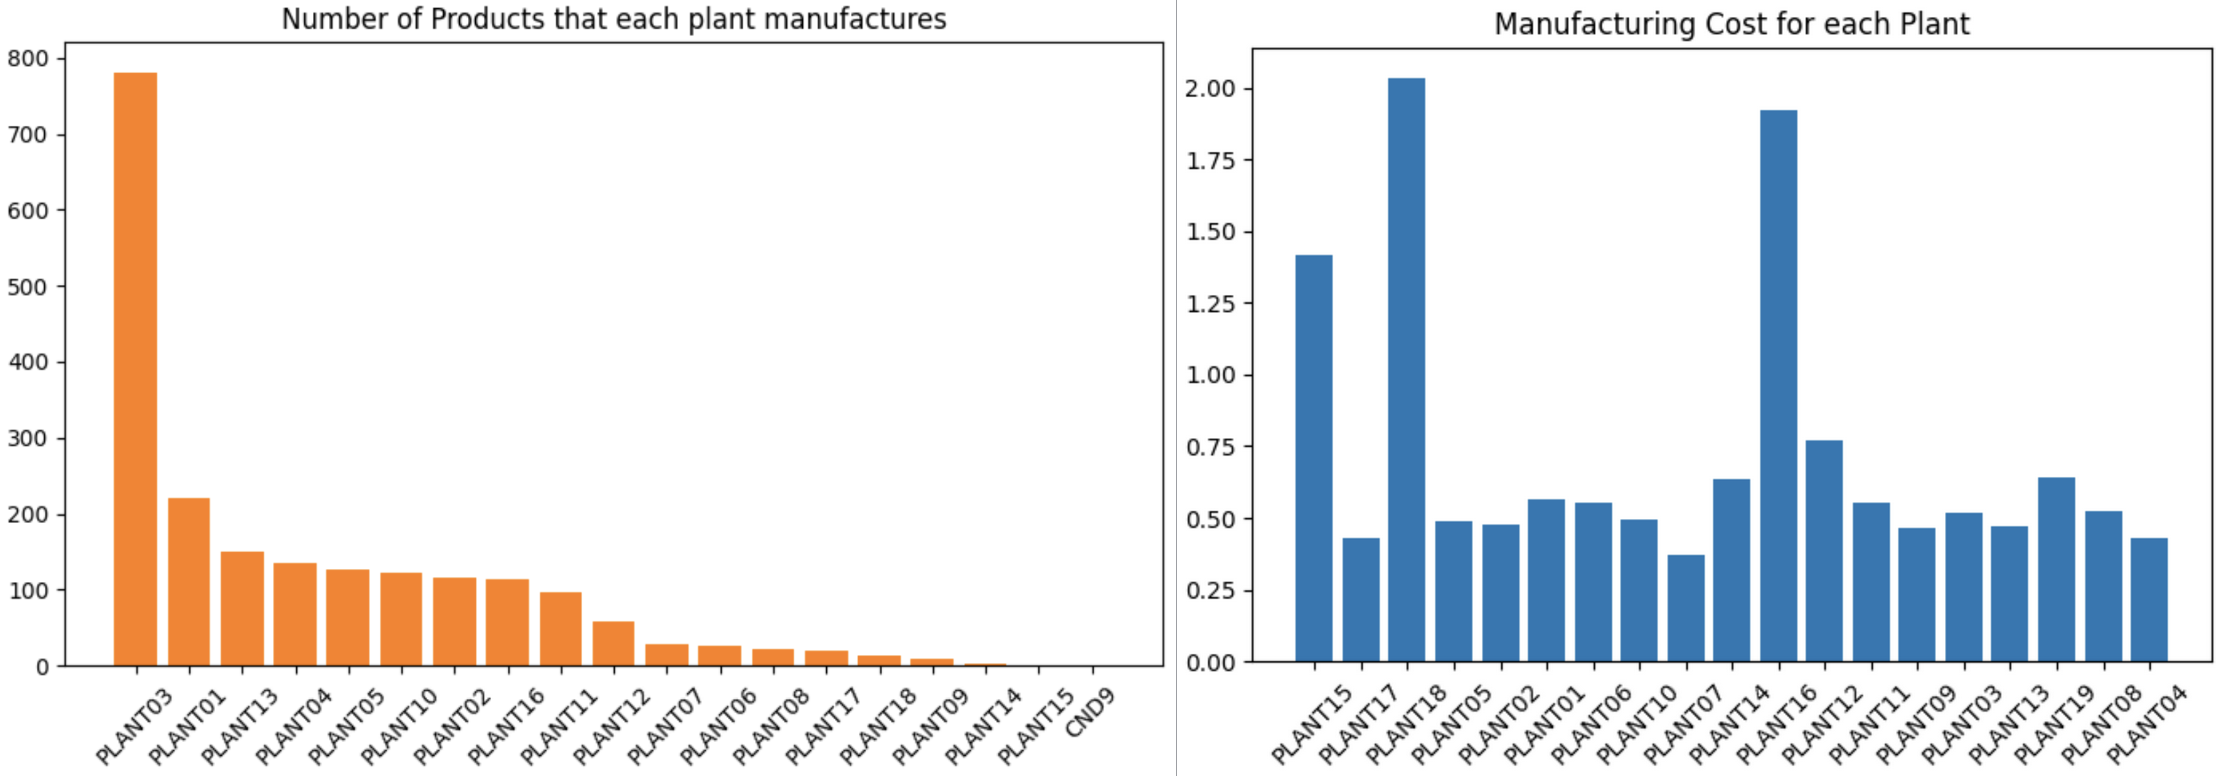
\includegraphics[width=0.7\paperwidth]{data_bar.png}
          \end{center}
     \caption{Number of products and manufacturing costs at each plant}
     \label{fig:cd}
\end{figure}


Exploratory data analysis was conducted to depict the relationships between key variables in the datasets. The correlation matrix for the \texttt{OrderList} data frame was calculated and visualized using a correlation heatmap. The analysis shows several remarkable and other questionable relationships between shipping costs, unit quantities, and various service levels. The average shipping rate and price elasticity from the \texttt{FreightRates} data frame were used to understand the pricing strategies adopted by carriers.

\section{Ideation}

Multiple ideas were assessed to absorb insights from the data:

\begin{itemize}
    \item \textbf{Service Level Distribution:} A count plot was used to examine the distribution of service levels across different orders.
    \item \textbf{Daily Capacity Distribution:} A boxplot was created to explore the distribution of daily capacities across various warehouses.
    \item \textbf{Weight vs. Shipping Cost:} A scatter plot was generated to understand how shipping costs vary with weight, colored by the carrier.
\end{itemize}

Additionally, a plot was generated to visualize the connections between \texttt{PlantCode} and \texttt{Port}, showing the logistics network and possible transportation routes between plants and ports.

\section{Optimization Model}

The optimization model was deployed as a MIP model. The objective was to minimize the total transportation cost by selecting the most cost-effective routes for delivering products from supply nodes (warehouses) to demand nodes (projects). However, one has to be sure about the passage through port 9, which is considered an obligatory constraint. 

\subsection{Decision Variables}

\begin{itemize}
    \item \textbf{Route Decision Variables:} A binary decision variable was created for each route, showing whether a particular supply-to-demand route is chosen.
\end{itemize}

\subsection{Objective Function}

The objective function is to minimize the total transportation cost, which is the sum of the transportation costs associated with each selected route. The objective function is given as:

\[
\text{Minimize } Z = \sum_{w \in W, b \in B} \text{cost}_{wb} \cdot x_{wb}
\]

Where:
\begin{itemize}
    \item \( \text{cost}_{wb} \) is the cost of transporting products from warehouse \( w \) to demand node \( b \),
    \item \( x_{wb} \) is a binary variable indicating whether the route from warehouse \( w \) to demand node \( b \) is selected.
\end{itemize}

\subsection{Constraints}

The optimization model is subject to several constraints:

\begin{figure}[!h]
     \begin{center}
     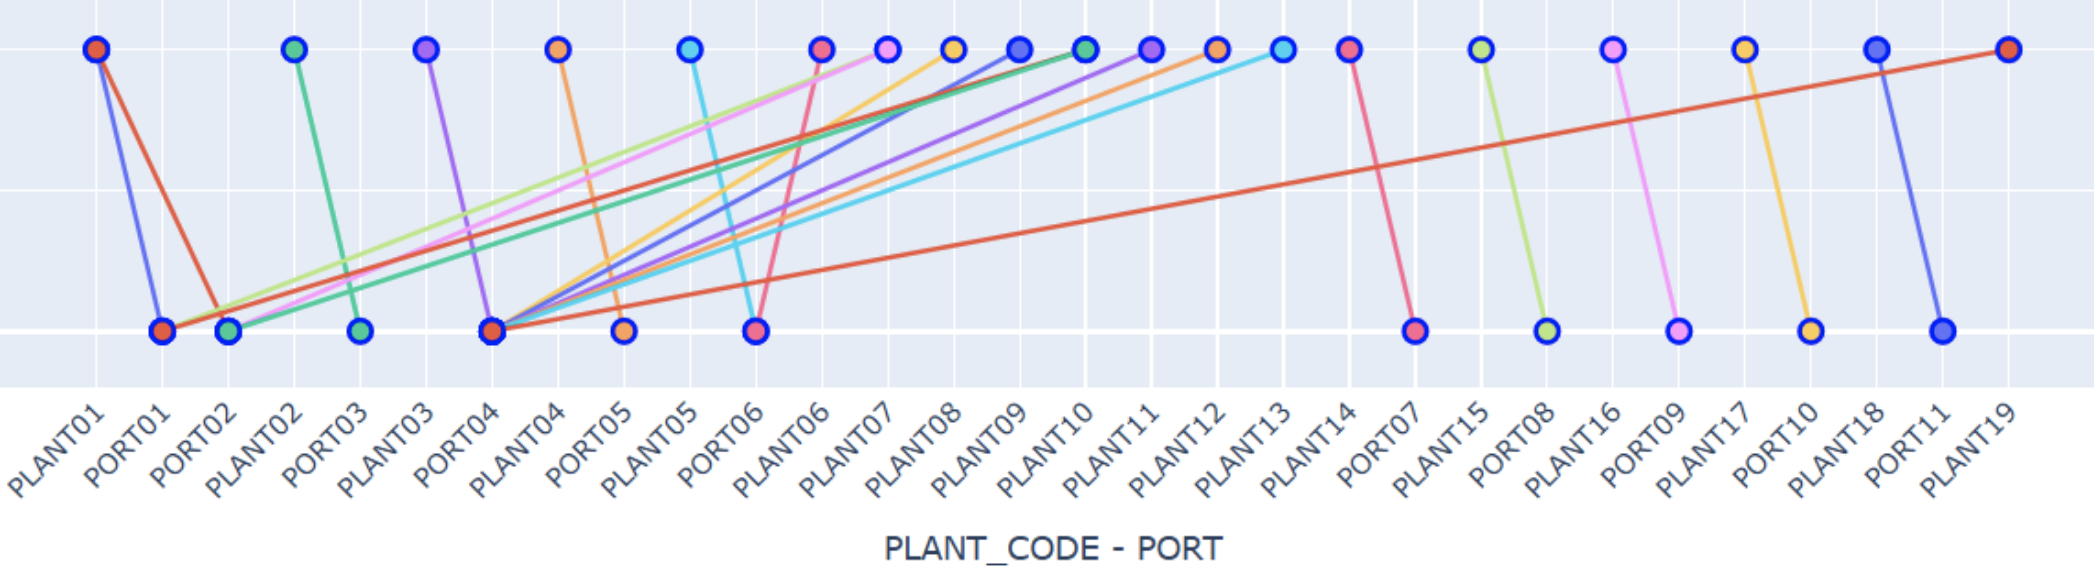
\includegraphics[width=0.6\paperwidth]{route.png}
          \end{center}
     \caption{Route constraints}
     \label{fig:cd}
\end{figure}


\begin{itemize}
    \item \textbf{Supply Constraints:} The total quantity shipped from a warehouse cannot exceed its supply capacity.
    \item \textbf{Demand Constraints:} The total quantity received at a demand node must meet or exceed its demand.
    \item \textbf{Self-Transportation Constraints:} Routes from a supply node to itself were excluded.
\end{itemize}

\section{Results}



The optimization was performed using the \texttt{Pulp} Python library, which solved the MIP problem using the default solver. The solution provided the optimal transportation routes and the associated costs. The following observations could be made:



\begin{table}[h!]
    \centering
    \begin{tabular}{|c|c|}
        \hline
        \textbf{Route} & \textbf{Value} \\
        \hline
        Route\_PLANT01\_PORT09 & 1070.0 \\
        Route\_PLANT02\_PORT09 & 138.0 \\
        Route\_PLANT03\_PORT09 & 555600470.0 \\
        Route\_PLANT04\_PORT09 & 554.0 \\
        Route\_PLANT05\_PORT09 & 385.0 \\
        Route\_PLANT06\_PORT09 & 49.0 \\
        Route\_PLANT07\_PORT09 & 265.0 \\
        Route\_PLANT08\_PORT09 & 14.0 \\
        Route\_PLANT09\_PORT09 & 11.0 \\
        Route\_PLANT10\_PORT09 & 118.0 \\
        Route\_PLANT11\_PORT09 & 332.0 \\
        Route\_PLANT12\_PORT09 & 209.0 \\
        Route\_PLANT13\_PORT09 & 490.0 \\
        Route\_PLANT14\_PORT09 & 549.0 \\
        Route\_PLANT15\_PORT09 & 11.0 \\
        Route\_PLANT16\_PORT09 & 457.0 \\
        Route\_PLANT17\_PORT09 & 8.0 \\
        Route\_PLANT18\_PORT09 & 111.0 \\
        Route\_PLANT19\_PORT09 & 7.0 \\
        \hline
    \end{tabular}
    \caption{Route Values for PORT09}
\end{table}


\begin{itemize}
    \item \textbf{Optimized Routes:} The optimization model identified the most cost-effective routes, considering both transportation and storage costs. Although it could not be optimal and feasible at the same time, the results show considerable promise. 
    \item \textbf{Total Cost:} The total cost of transportation for all orders was minimized, leading to a reduction in overall logistics expenses. However, there are some uncertainties associated with most likely discontinued ports and so on. Further data enhancement is required to overcome this. Final cost: \textbf{6821943477.0432}
\end{itemize}


\section{Conclusion}

This optimization approach demonstrates the potential for significant cost savings in supply chain logistics through route optimization. By integrating supply and demand data, freight rates, and warehouse capacities, the optimization model identifies the most efficient routes to minimize transportation costs. The model's results can be used for better decision-making in material supply management, contributing to enhanced supply chain performance.

Future improvements can be made if more robust data can be obtained. More sophisticated models could also enhance the performance; however, such things should be tested beforehand.


\end{document}